\documentclass[aps,twocolumn]{revtex4-1} 

\usepackage{amsmath}  % needed for \tfrac, \bmatrix, etc.
\usepackage{amsfonts} % needed for bold Greek, Fraktur, and blackboard bold
\usepackage{graphicx} % needed for figures


\begin{document}

\title{Newton's Cannon Simulation with Hamiltonian Mechanics}


\author{Oscar Jaroker}
%\affiliation{Department of Physics \& Astronomy, Colgate University, Hamilton, NY 13346}


\date{\today}

\begin{abstract}
Newton's Cannon is a famous thought experiment that illustrates the effects of universal gravitation as it relates to orbital motion. First appearing in Newton's posthumously published \textit{De mundi systemate}, Newton correctly hypothesizes the trajectories of stones launched horizontally from the top of a mountain, where increasing velocity increases the distance the stone travels before it may or may not impact the Earth. Many methods exist to model the trajectory of such a stone, mostly using Newton's Laws of Motion. This paper demonstrates an alternative approach using Hamilton's equations and representing the two-dimensional system in polar coordinates. A \verb|MATLAB| simulation using the discussed approach confirms the 17th-century hypotheses of Newton's illustration. 

\end{abstract}

\maketitle 

\section{Introduction} 
\begin{figure}
    \centering
    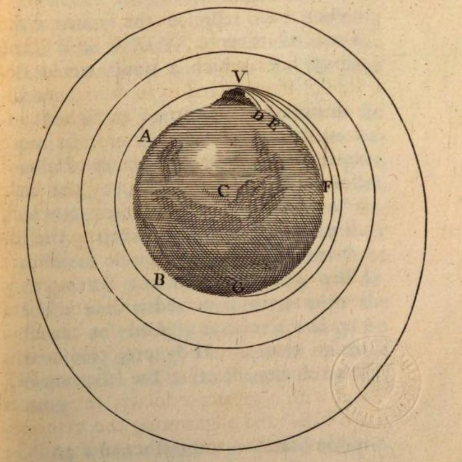
\includegraphics[width=0.5\linewidth]{newtonDiagram.png}
    \caption{Original illustration of Newton's Cannon from \textit{De mundi systemate} \cite{Newton} showing trajectories at different velocities of a stone launched from a tall mountain.}
    \label{newtonFig}
\end{figure}
Projectile motion is a fundamental application of physics, studied extensively by Newton as evidence for the existence of a gravitational force. In the first sections of Newton's \textit{De mundi systemate}, translated and published after his death as \textit{A Treatise of the System of the World}, Newton illustrates his claims with a diagram, see Fig. \ref{newtonFig}. Newton argues that the ``perpetual deflection" (gravitation) towards the Earth of a stone launched horizontally from atop a tall mountain, in the absence of air, is evidence of a force in the direction of the center of the Earth. However, with sufficient initial velocity, the stone will continue to accelerate in the direction of the Earth but will never reach the surface, returning to the mountain top from which it was projected \cite{Newton}.

Deriving the stone's equations of motion using Newton's Second Law and force analysis results in second-order differential equations that prove quite challenging to solve analytically. These formidable equations are introduced in this situation by the particle's motion occurring under the constraint of a gravitational force.  Past simulations\cite{noragulfa} of this thought experiment use numerical methods such as Euler-Cromer or Runge-Katta processes.

Hamiltonian mechanics reformulates Newtonian mechanics, describing systems by energy rather than forces. It expresses motion with position and momentum rather than acceleration. Hamilton's equations reduce the second-order differential equations of motion to multiple first-order equations, allowing for a more conceptual understanding of the system.

\section{Describing the System}
Newton's illustration is extremely conceptual, depicting a mountain that rises around 1000 kilometers above sea level (For reference, Mt. Everest\cite{everest} is about 8.8 km. tall). To remain consistent with the original diagram, a height of 1000 kilometers will be the starting point of the stone, equivalent to 7371 kilometers from the center of the Earth. This experiment assumes the Earth to be spherical and uses its mean radius\cite{meanRadius}, $R_E=6371$ km. As is true with most two-dimensional systems with circular elements, changing to polar coordinates simplifies calculations. Define $\theta=0$ as the equator (right side), increasing in the counter-clockwise direction, so the stone's initial $\theta$ is $\pi/2$.

Now define the stone's kinetic and potential energies of $T=mv^2/2$ and $V=-GmM_E/r$, respectively, where the Earth has mass $M_E$.

\section{A Newtonian Approach}
Before demonstrating the Hamiltonian approach, it is worthwhile to consider how Newton would perform the same exercise.

The system will be represented with polar coordinates to remain consistent with the alternative approach. In the two-body system, the only force present is due to gravitational attraction, which is a central force. For the stone of mass $m$, by Newton's second law:
\begin{equation}
    \sum\Vec{F}_{r} = -\frac{GM_Em}{r^2}e_r = m\Vec a_r
\end{equation}
\begin{equation}
    \sum\Vec{F}_\theta = 0 = ma_\theta
\end{equation}

Where $e_r$ is a unit vector pointing in the direction of increasing radial distance from the center of the Earth and $e_r=\cos{\theta} \hat{i} + \sin{\theta}\hat{j}$. It may be shown that radial acceleration $a_r=\Ddot{r}-r\dot{\theta}^2$ and angular acceleration $a_\theta = r\Ddot \theta + 2\dot r \dot \theta$ (See Appendix for derivation). Dividing both sides by $m$ leaves:
\begin{equation}
    -\frac{GM_E}{r^2} = \Ddot r - r\dot \theta^2
\end{equation}
\begin{equation}
    0 = r\Ddot \theta + 2\dot r \dot \theta
\end{equation}

Solving this system of differential equations may be an exercise for another time\cite{orbitSolution}.

\section{Hamiltonian Approach: Equations of Motion}
In a system with time-independent coordinates, $q$, as $r$ and $\theta$ are in this example, the Hamiltonian $H$ represents the total energy of the system in terms of $q$ and momenta $p$.
\begin{equation}
    H = \sum_{i} p_i\dot q_i - L
\end{equation}

Where $L$ is the Lagrangian and is defined as the difference in kinetic and potential energy. Hamilton's equations express motion in terms of position and momentum and are defined as:
\begin{equation}
    \dot q_i = \frac{\partial H}{\partial p_i} \label{qdot}
\end{equation}
\begin{equation}
    \dot p_i = -\frac{\partial H}{\partial q_i} \label{pdot}
\end{equation}

First, define the Hamiltonian for the system in polar coordinates:
\begin{equation*}
    H=p_r\dot r + p_{\theta}\dot \theta - (T-V)
\end{equation*}
\begin{equation*}
    H =p_r\dot r + p_{\theta}\dot \theta - \frac{1}{2}mv^2 - \frac{GM_Em}{r}
\end{equation*}

$v^2$ becomes $\dot r^2 + r^2 \dot \theta^2$ (See Appendix for derivation), and distribute terms.
\begin{equation}
        H =p_r\dot r + p_{\theta}\dot \theta - \frac{1}{2}m\dot r^2 - \frac{1}{2}m r^2 \dot \theta^2 - \frac{GM_Em}{r}
\end{equation}

Now express all terms except for potential energy with $p_i^2$, remembering radial momentum $p_r=m\dot r$ and angular momentum for a point mass (stone) $p_\theta = mr^2\dot \theta$:
\begin{equation*}
    H = \frac{p_r^2}{m} + \frac{p_\theta^2}{mr^2} - \frac{p_r^2}{2m} - \frac{p_\theta^2}{2mr^2} - \frac{GM_Em}{r}
\end{equation*}
\begin{equation}
    H = \frac{p_r^2}{2m} + \frac{p_\theta^2}{2mr^2} - \frac{GM_Em}{r} \label{energyH}
\end{equation}

Use the Hamiltonian\footnote{Note: In equation \ref{energyH}, $H$ expresses the system's total energy $T + V$.} with equations \ref{qdot} and \ref{pdot} to find the four first-order equations of motion:

\begin{equation}
    \dot r = \frac{p_r}{m} 
\end{equation}
\begin{equation}
    \dot \theta = \frac{p_\theta}{mr^2} 
\end{equation}
\begin{equation}
    \dot p_r = \frac{p_\theta^2}{mr^3} - \frac{GM_Em}{r^2}
\end{equation} 
\begin{equation}
    \dot p_\theta  = 0
\end{equation}

These four equations\footnote{Note: The equation for $\dot p_r$ is consistent with the definition of force $F_r=\dot p_r = m\Ddot{r}$ when treating the object as a point mass ($I=MR^2$). $\dot p_\theta = 0$ is consistent with the conservation of angular momentum in this system, where net torque is zero.}, along with the initial conditions for the system, may be solved numerically to find the trajectory of the stone. 

\section{Simulation Design}
One can simulate the motion of the stone with Simulink in \verb|MATLAB|. Initial conditions for the system are as follows:
\begin{align*}
    p_r(0) &= 0\\
    r(0) &= R_E+h\\
    p_\theta &= (R_E+h)mv_0\\
    \theta(0)&=\frac{\pi}{2}
\end{align*}

\begin{figure}
    \centering
    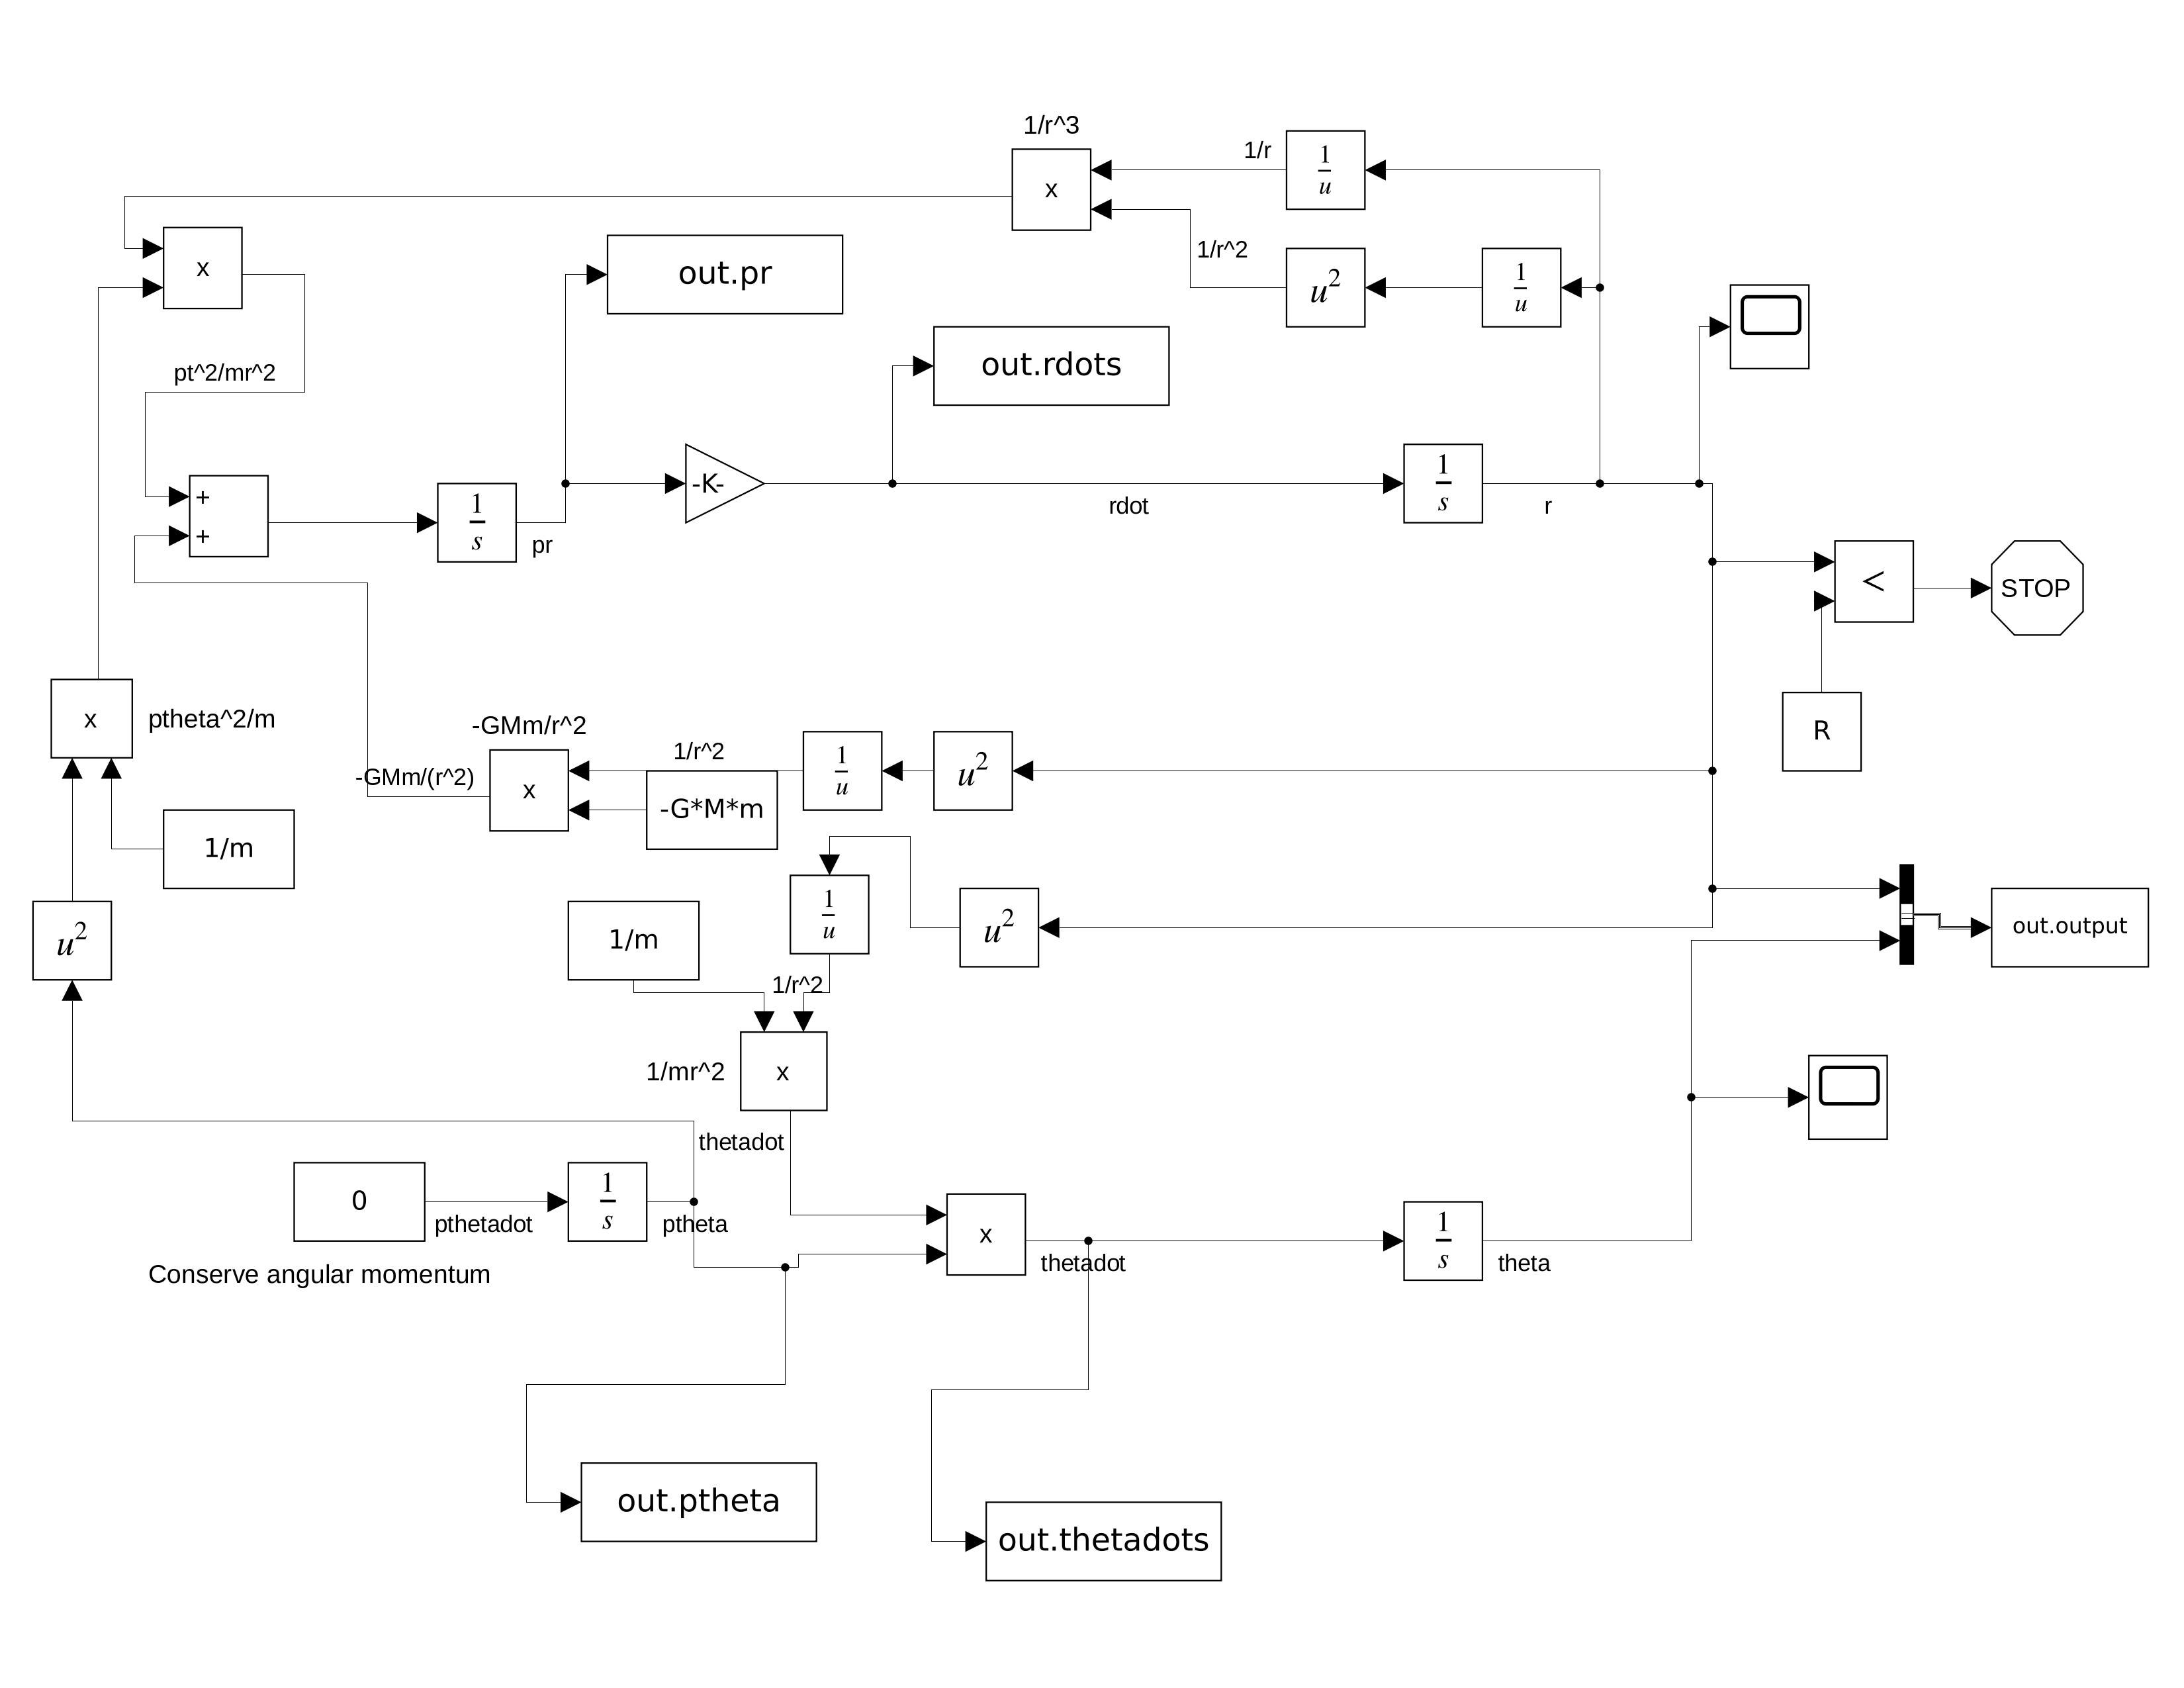
\includegraphics[width=.5\textwidth]{projectile.jpg}
    \caption{Simulink Model for Projectile}
    \label{simulink}
\end{figure}
Figure \ref{simulink} shows a Simulink model used to calculate $r$ and $\theta$ values. To numerically solve the differential equations, this model starts with time derivatives of the generalized momenta ($\dot p_r, \dot p_\theta$) and uses integrator blocks to eventually solve for $r$ and $\theta$. The \verb|ode4| solver with a Runge-Katta method with a fixed step size of 5 seconds is used to achieve a smooth curve. Finally, every calculated value, $r,\theta,\dot{r},\dot{\theta},p_r,p_\theta$ is returned as output to the \verb|MATLAB| workspace, where results may be analyzed. Note that after all calculations, the trajectory of the stone is independent of its mass $m$.

\section{Results}
\begin{figure}
    \centering
    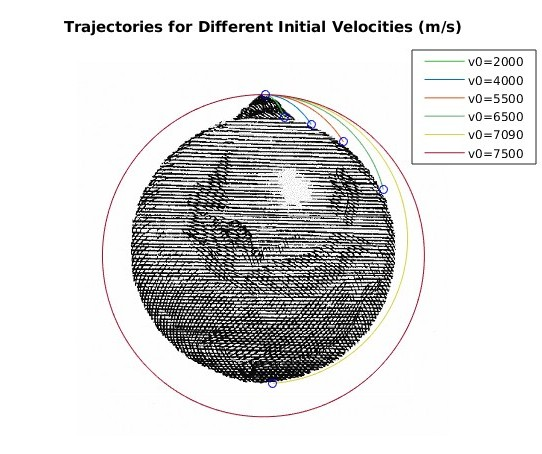
\includegraphics[width=.5\textwidth]{diffTrajec.jpg}
    \caption{Trajectories at Different Initial Velocities}
    \label{diffTrajec}
\end{figure}
Changing initial velocity values leads the projectile to travel further around the Earth, eventually entering orbit with an initial velocity of around $7090$ m/s, confirming Newton's hypotheses. Figure \ref{diffTrajec} shows trajectories of the projectile for different initial velocities, where the object will land on the Earth's surface for initial speeds less than around $7090$ m/s, and enter a circular orbit for initial speeds around $7500$ m/s \footnote{Note: This speed is consistent with calculations for Low Earth Circular Orbits, $v=\sqrt{\frac{GM}{R}}$.}. 
\begin{figure}
    \centering
    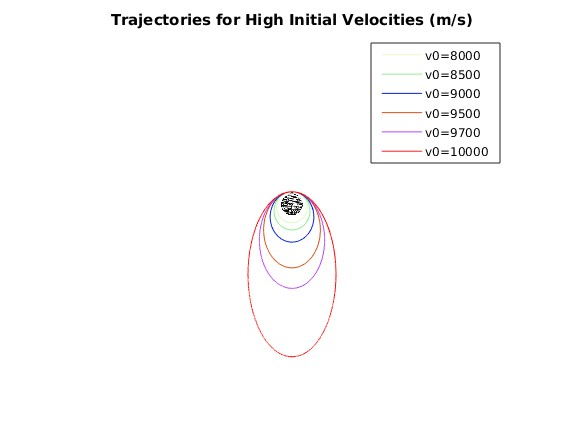
\includegraphics[width=.5\textwidth]{highVelo.jpg}
    \caption{Trajectories at High Velocities}
    \label{highVelo}
\end{figure}

At high velocities, the eccentricity of the orbit increases and the elliptical path flattens. Figure \ref{highVelo} extends the velocities shown in Figure \ref{diffTrajec} and zooms out by a factor of 10. Still, the orbiting object returns to its starting point, no matter the initial speed. Note that the stop time for the simulation must be raised as the initial velocity increases.

\section{Conclusion}
This paper demonstrates a numerical method for solving for the trajectory of an object under the influence of a central force, such as that of gravity, using Hamiltonian Mechanics. It discusses the differences between Newton's and Hamilton's approaches and force versus energy analysis.

Many simplifications are made in this exercise, most notably the disregard for the Earth's atmosphere and the orbital decay it causes. However, because the launch height is so high (in the exosphere), the air density is so low that the lifetime of such an orbit would be measured in centuries \cite{nasaDecay}.

\verb|MATLAB|'s Simulink and \verb|ode4| are used to numerically solve the equations of motions, and an accompanying script plots the trajectories over the image of the Earth that Newton drew in \textit{De mundi systemate}.


\newpage
\appendix  

\section{Acceleration in Polar Coordinates}
Show $a_r = \Ddot{r}-r\dot{\theta}^2$ and $a_\theta = r\Ddot \theta + 2\dot r \dot \theta$
\begin{equation*}
    e_r = \cos{\theta} \hat{i} + \sin{\theta}\hat{j},   \quad  
    e_\theta = -\sin{\theta}\hat{i} + \cos{\theta}\hat{j}
 \tag{Define Standard Unit Vectors}
\end{equation*}
Given position $\Vec{r} = re_r$:
\begin{equation*}
    v = \dot r = \dot r e_r  + r \dot e_r = \dot r\cos{\theta} \hat{i} + \dot r\sin{\theta}\hat{j} - r \dot \theta \sin{\theta}\hat{i} + r\dot \theta \cos{\theta}\hat{j} \tag{Differentiate Position Vector}
\end{equation*}
\begin{equation*}
    v = \dot r e_r + r\dot \theta e_\theta \tag{Simplify}
\end{equation*}
\begin{equation*}
    a = \Ddot r e_r + \dot r \dot e_r + \dot r \dot \theta e_\theta + r \Ddot{\theta} e_\theta + r \dot \theta \dot e_\theta \tag{Differentiate Velocity Vector}
\end{equation*}
Use chain rule:
\begin{equation*}
\dot e_r = \frac{de_r}{dt} = \frac{de_r}{d\theta}\frac{d\theta}{dt}, \quad \dot e_\theta = \frac{de_\theta}{dt} = \frac{de_r}{d\theta}\frac{d\theta}{dt}
\end{equation*}
Note:
\begin{equation*}
    \frac{de_r}{d\theta} = e_\theta, \quad \frac{de_\theta}{d\theta} = -e_r
\end{equation*}
\begin{equation*}
    a = \Ddot{r} e_r + \dot r \dot \theta e_\theta + \dot r \dot \theta e_\theta + r \Ddot \theta e_\theta - r \dot \theta^2 e_r \tag{Substitute}
\end{equation*}
\begin{equation*}
    a_r = \Ddot r - r\dot \theta^2 \tag{Group $e_r$ Terms}
\end{equation*}
\begin{equation*}
    a_\theta = r\Ddot \theta + 2\dot r \dot \theta \tag{Group $e_\theta$ Terms}
\end{equation*}



\section{Squared Velocity in Polar Coordinates}
Show $v^2 = \dot x^2 + \dot y^2 = \dot r^2 + r^2 \dot \theta^2$:
\begin{equation*}
    x=r\cos{\theta}, \quad y=r\sin{\theta} \tag{Change of Coordinates}
\end{equation*}
\begin{equation*}
    \dot x = \dot r\cos{\theta} - r\dot \theta \sin{\theta}, \quad
    \dot y = \dot r\sin{\theta} + r\dot \theta \cos{\theta}
    \tag{Chain Rule}
\end{equation*}
\begin{equation*}
    \dot x^2 = \dot r^2\cos^2\theta-2\dot r r \dot \theta  \sin{\theta} \cos{\theta} + r^2 \dot \theta^2\sin^2\theta
\end{equation*}
\begin{equation*}
    \dot y^2 = \dot r^2\sin^2\theta + 2\dot r r \dot \theta  \sin{\theta} \cos{\theta} + r^2 \dot \theta^2\cos^2\theta
\end{equation*}
\begin{equation*}
    \dot x^2 + \dot y^2 = \dot r^2\cos^2\theta + r^2 \dot \theta^2\sin^2\theta + \dot r^2\sin^2\theta +  r^2 \dot \theta^2\cos^2\theta \tag{Combine}
\end{equation*}
\begin{equation*}
    v^2 = \dot x^2 + \dot y^2 = \dot r^2 + r^2 \dot \theta^2 \tag{Pythagorean Identity}
\end{equation*}

\section{MATLAB Code}
\begin{verbatim}
m=1; % mass of projectile (irrelevant) (kg)
R=6371000; % mean radius of earth (m)
startHeight = .155*R; % height, abt 1000 km
G=6.6743e-11; % gravitational constant (Nm^2/kg^2)
M=5.97219e24; % mass of earth (kg)
v0 = 7000; % launch speed (m/s)
scaleFactor = 1e4;

hold on
% load and scale image
img = imread("NewtonWorld.png");
img = imresize(img, [1770,1770]);
img = flipdim(img,1);
% center image
imshow(img, 'XData', [-883, -883 + size(img,2)], ...
    'YData', [-884, -884 + size(img,1)]);

% change axis scale. 1e3 default.
axis([-1e3 1e3 -1e3 1e3])
% make pi/2 top and positive velocity clockwise
set(gca,'XDir','reverse','YDir','normal') 
axis equal
% white background
set(gcf,'Color','w')

v0vals = [4000 5000 6000 7000 7200 7500];
% endVals for plotting points at stopping location
% endVals = zeros(6,2);
counter=1;
for i = v0vals
    v0 = i;
    % get simulated trajectory values r,theta
    % Simulink file at github.com/ojaroker/Projectile
    out = sim('projectile.slx');
    rVals = out.output(:,1);
    thetaVals = out.output(:,2);
    % convert to cartestian, scale
    xVals = rVals .* cos(thetaVals) ./ scaleFactor;
    yVals = rVals .* sin(thetaVals) ./ scaleFactor;
    % instant plotting:
    plot(xVals,yVals,'Color',rand(1,3))
    % endVals(counter,1) = xVals(end);
    % endVals(counter,2) = yVals(end);
    % comet for animation:
    % comet(xVals,yVals,.3)
    counter = counter + 1;
end
legend(char(['v0=' int2str(v0vals(1))]), ...
    char(['v0=' int2str(v0vals(2))]), ...
    char(['v0=' int2str(v0vals(3))]), ...
    char(['v0=' int2str(v0vals(4))]), ...
    char(['v0=' int2str(v0vals(5))]), ...
    char(['v0=' int2str(v0vals(6))]))
title(['Trajectories for ' ...
    'Different Initial Velocities (m/s)'])
hold off
\end{verbatim}

\begin{thebibliography}{9}

% https://books.google.com/books?id=rEYUAAAAQAAJ&printsec=frontcover&source=gbs_ge_summary_r&cad=0#v=twopage&q&f=false
\bibitem{Newton} Isaac Newton, \textit{A Treatise of the System of the World}. (London, 1728), pp. 3-8.

\bibitem{noragulfa} Geoff Nunes, Newton's Cannon v2.12. \url{https://noragulfa.com/cannon/}.

\bibitem{everest} National Geographic, Mount Everest. \url{https://education.nationalgeographic.org/resource/mount-everest/}.

\bibitem{meanRadius} NASA, Earth Fact Sheet. \url{https://nssdc.gsfc.nasa.gov/planetary/factsheet/earthfact.html}.

\bibitem{orbitSolution} Kurt Toman, ``Central-Force Laws for an Elliptic Orbit." \textit{The American Mathematical Monthly}, vol. 71, no. 1, 1964, pp. 58–60.

\bibitem{nasaDecay} NASA, Orbital Debris Program Office FAQ. \url{https://orbitaldebris.jsc.nasa.gov/faq/}.

\end{thebibliography}

\end{document}
